\section{Assignment 2}

\subsection{Implement the three two-channel bilateral teleoperation architectures and the three-channel bilateral teleoperation architecture}

The three two-channel architectures and the three channel architecture are obtained by removing some of the coordinating controllers:

\begin{itemize}
\item 2-channel position-position (P-P): $C_2=C_3=0$
\item 2-channel force-position (F-P): $C_3=C_4=0$
\item 2-channel force-force (F-F): $C_1=C_4=0$
\item 3-channel position and force-position (P,F-P): $C_3=0$
\end{itemize}

The four architectures are modelled with the same SIMULINK model, which is based on the 4-channel architecture, with the added possibility of individually cutting off the coordinating controllers:

\begin{figure}[H]
\centering
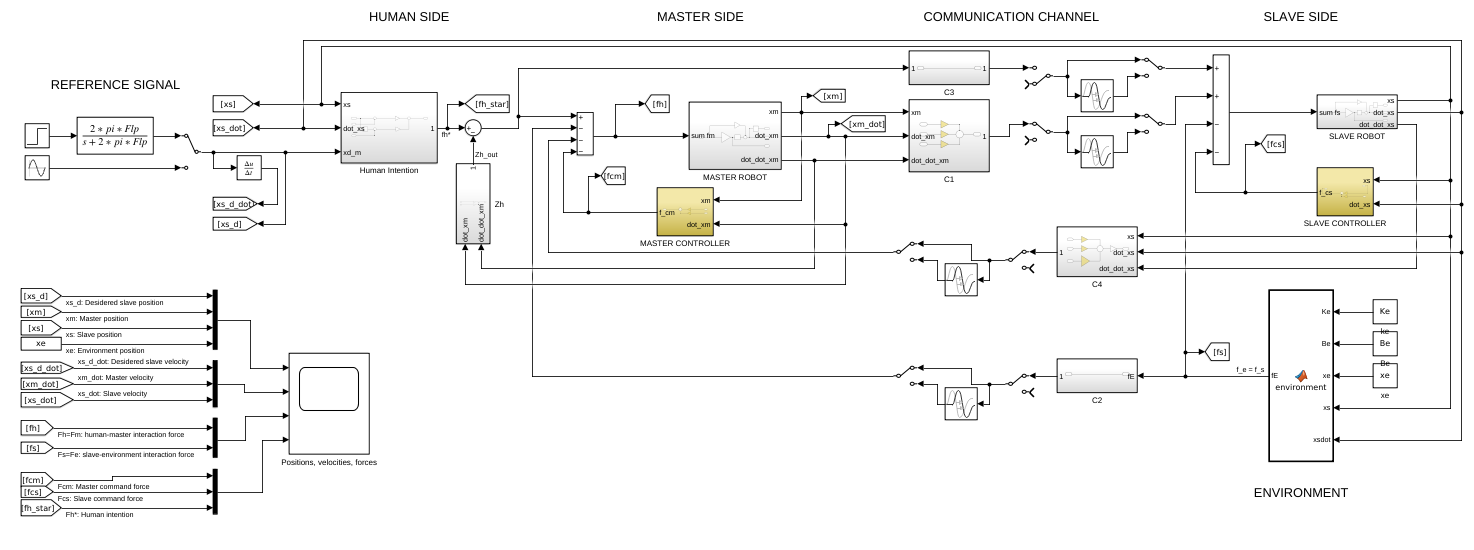
\includegraphics[keepaspectratio,width=0.9\textwidth]{2_3_ch_arch}
\caption{2-3 channel teleoperation architecture with transport delays - SIMULINK model}
\end{figure}

\newpage

\begin{figure}[H]
\begin{minipage}{0.5\textwidth}
\begin{figure}[H]
\centering
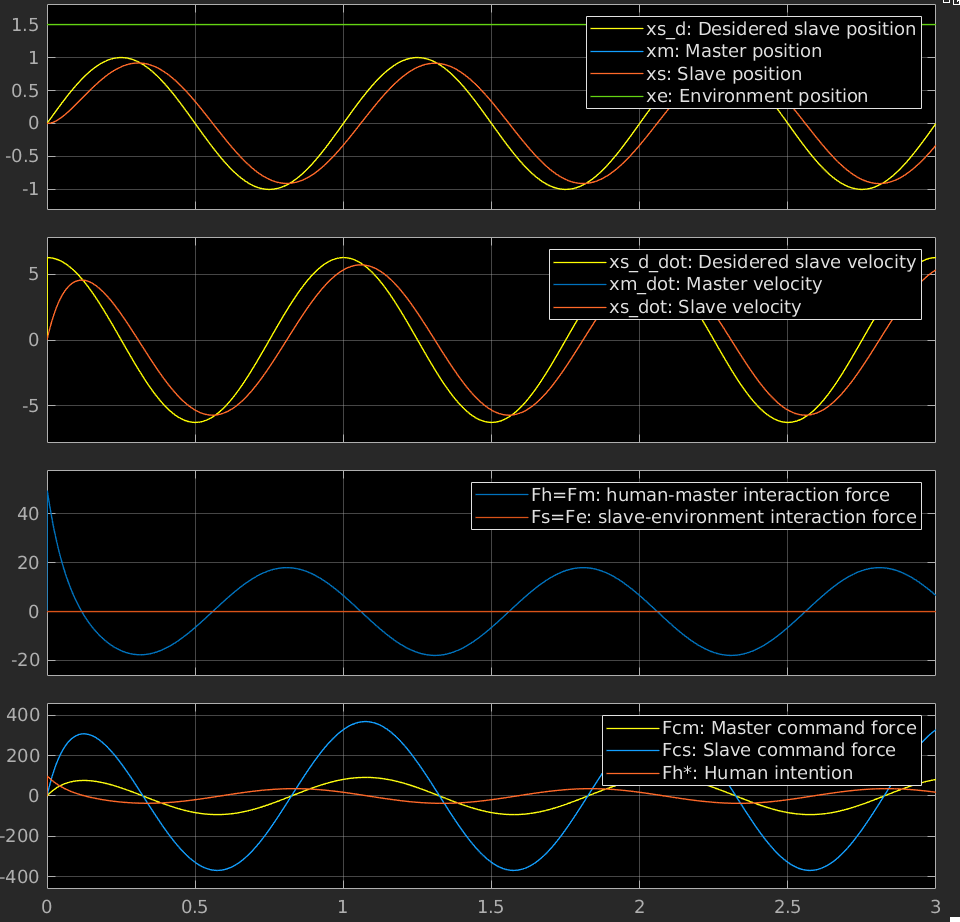
\includegraphics[keepaspectratio,width=\textwidth]{PP_free_nod}
\caption{2-channel P-P in free motion.}
\label{fig:pp_free}
\end{figure}
\begin{figure}[H]
\centering
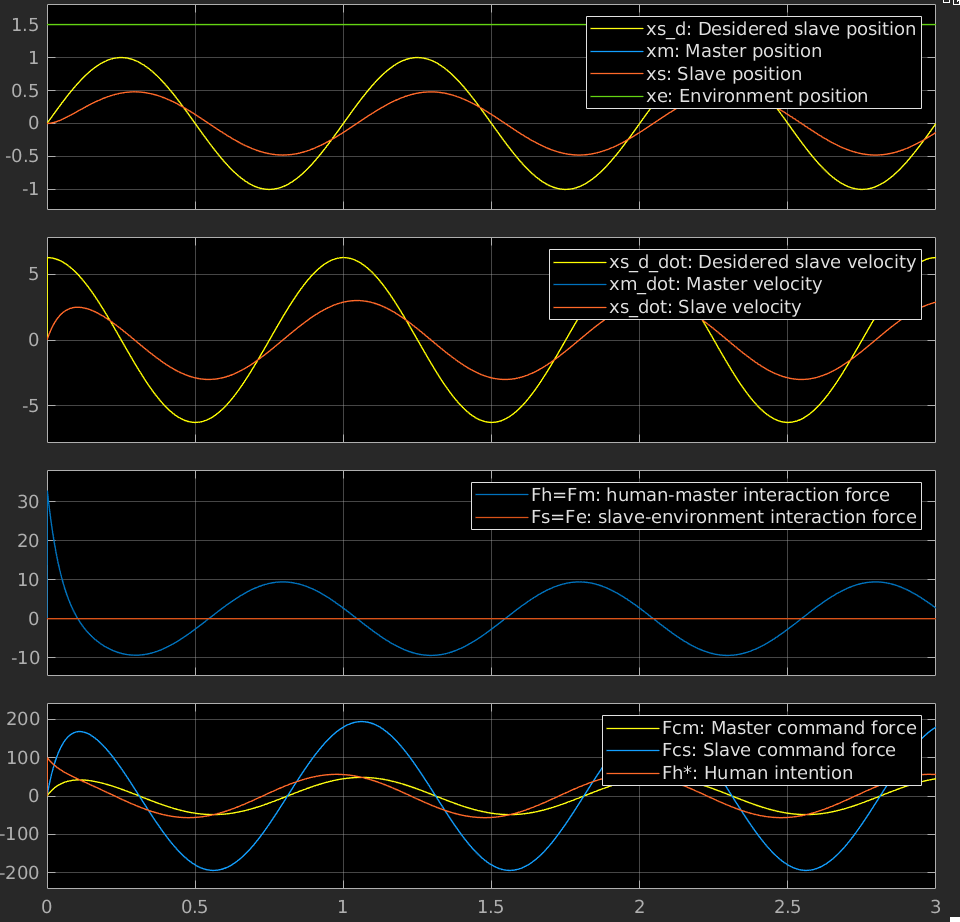
\includegraphics[keepaspectratio,width=\textwidth]{FP_free_nod}
\caption{2-channel F-P in free motion.}
\label{fig:fp_free}
\end{figure}
\end{minipage}
\begin{minipage}{0.5\textwidth}
\begin{figure}[H]
\centering
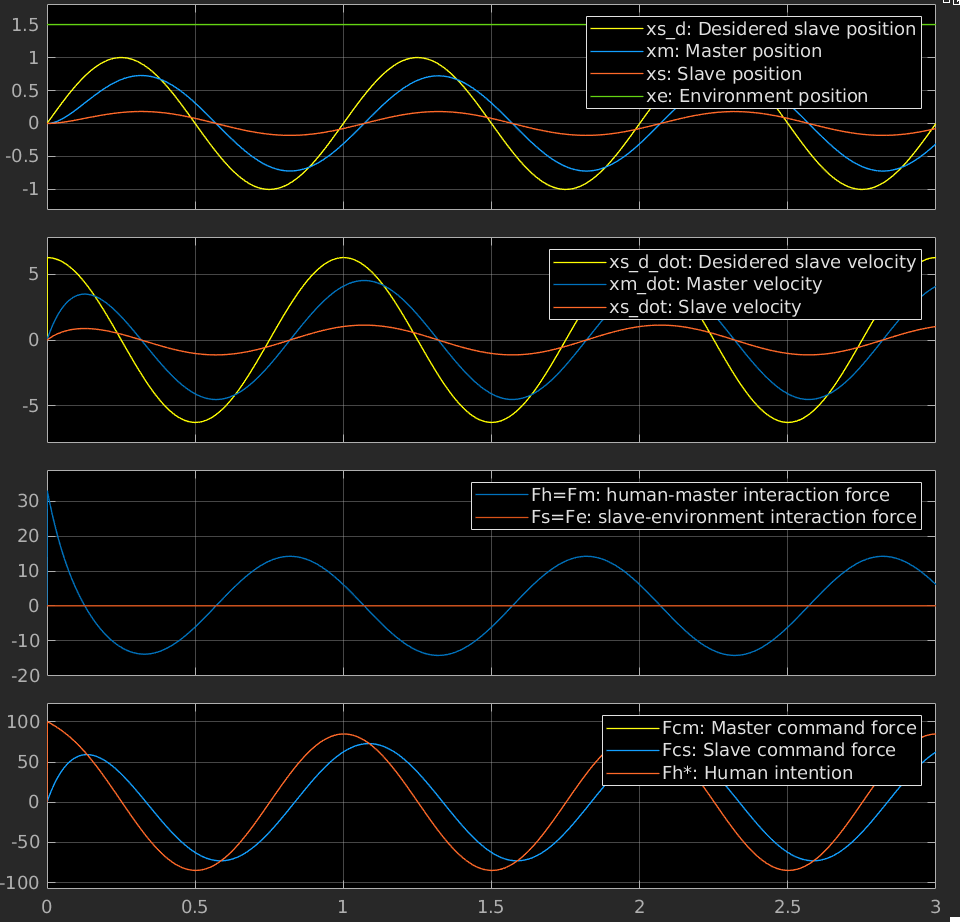
\includegraphics[keepaspectratio,width=\textwidth]{FF_free_nod}
\caption{2-channel F-F in free motion.}
\label{fig:ff_free}
\end{figure}
\begin{figure}[H]
\centering
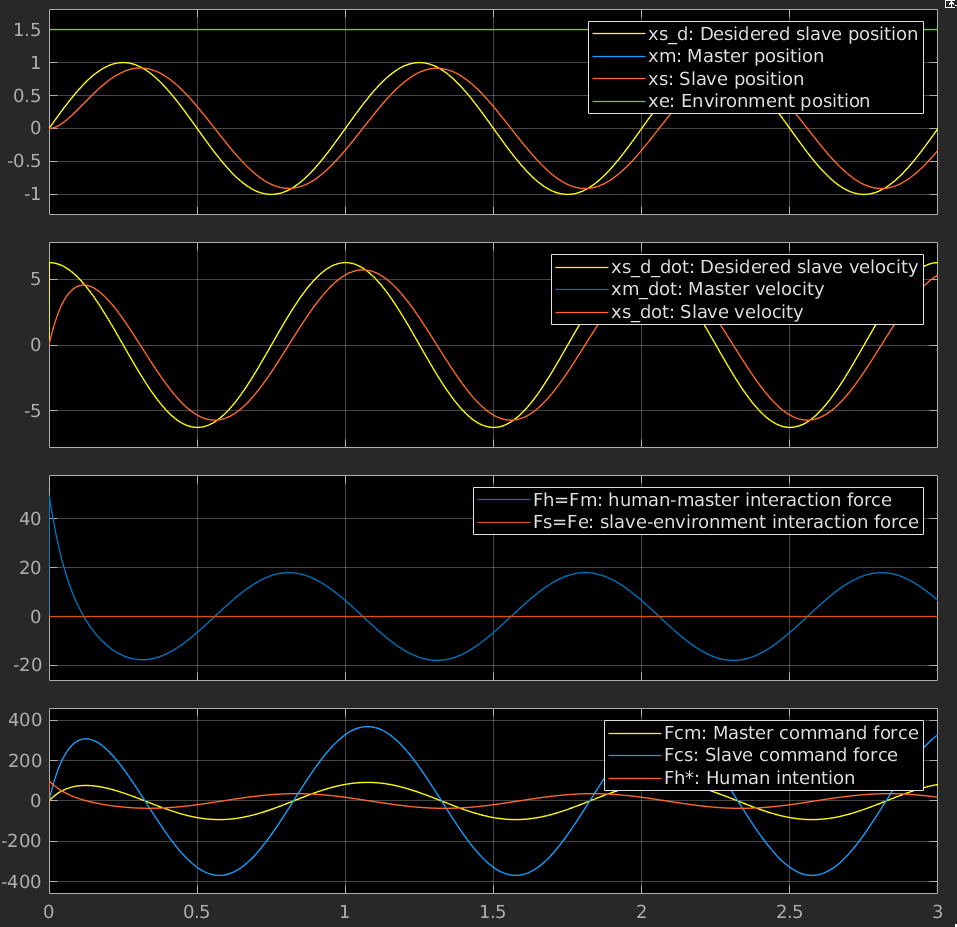
\includegraphics[keepaspectratio,width=\textwidth]{PFP_free_nod}
\caption{3-channel P,F-P in free motion.}
\label{fig:pfp_free}
\end{figure}
\end{minipage}
\end{figure}

\newpage

\begin{figure}[H]
\begin{minipage}{0.5\textwidth}
\begin{figure}[H]
\centering
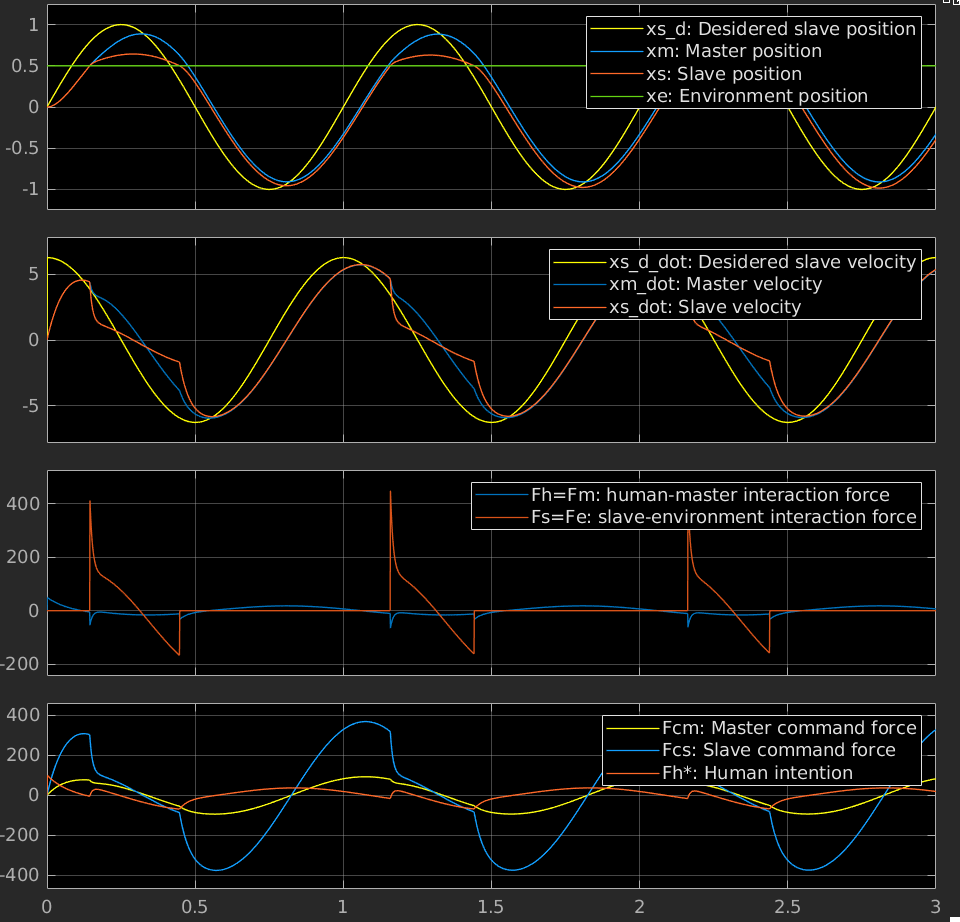
\includegraphics[keepaspectratio,width=\textwidth]{PP_contact_nod}
\caption{2-channel P-P in contact.}
\label{fig:pp_contact}
\end{figure}
\begin{figure}[H]
\centering
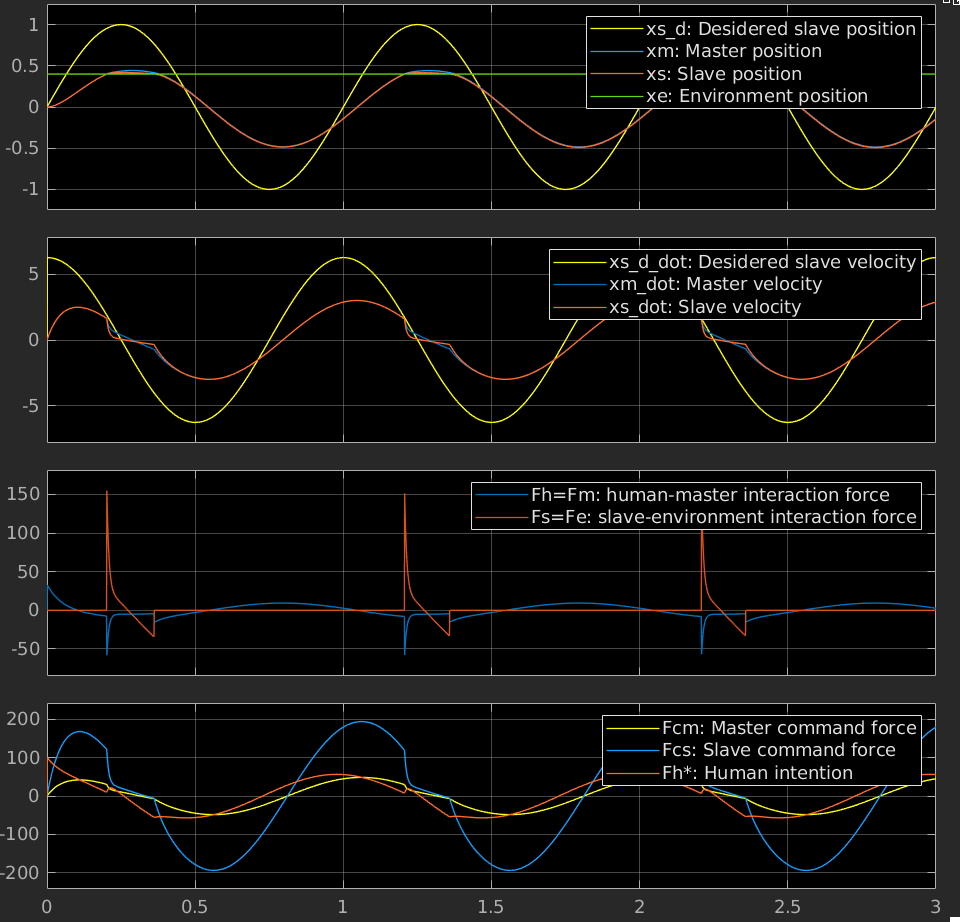
\includegraphics[keepaspectratio,width=\textwidth]{FP_contact_nod}
\caption{2-channel F-P in contact.}
\label{fig:fp_contact}
\end{figure}
\end{minipage}
\begin{minipage}{0.5\textwidth}
\begin{figure}[H]
\centering
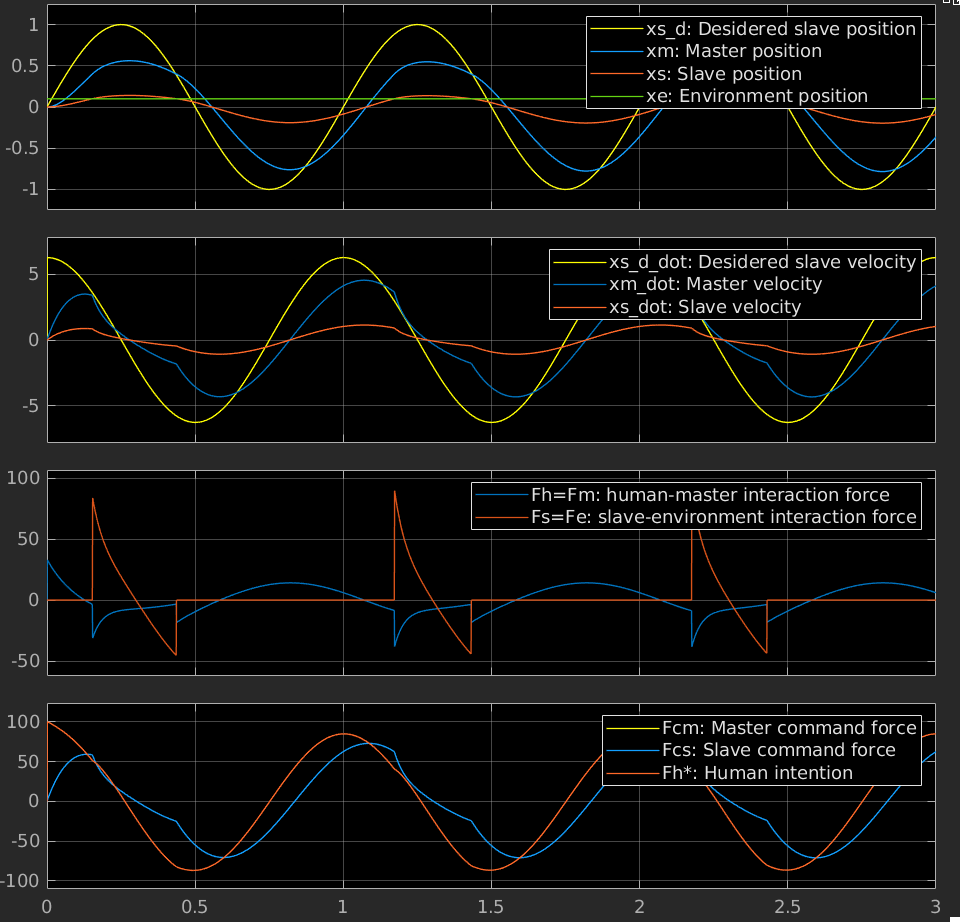
\includegraphics[keepaspectratio,width=\textwidth]{FF_contact_nod}
\caption{2-channel F-F in contact.}
\label{fig:ff_contact}
\end{figure}
\begin{figure}[H]
\centering
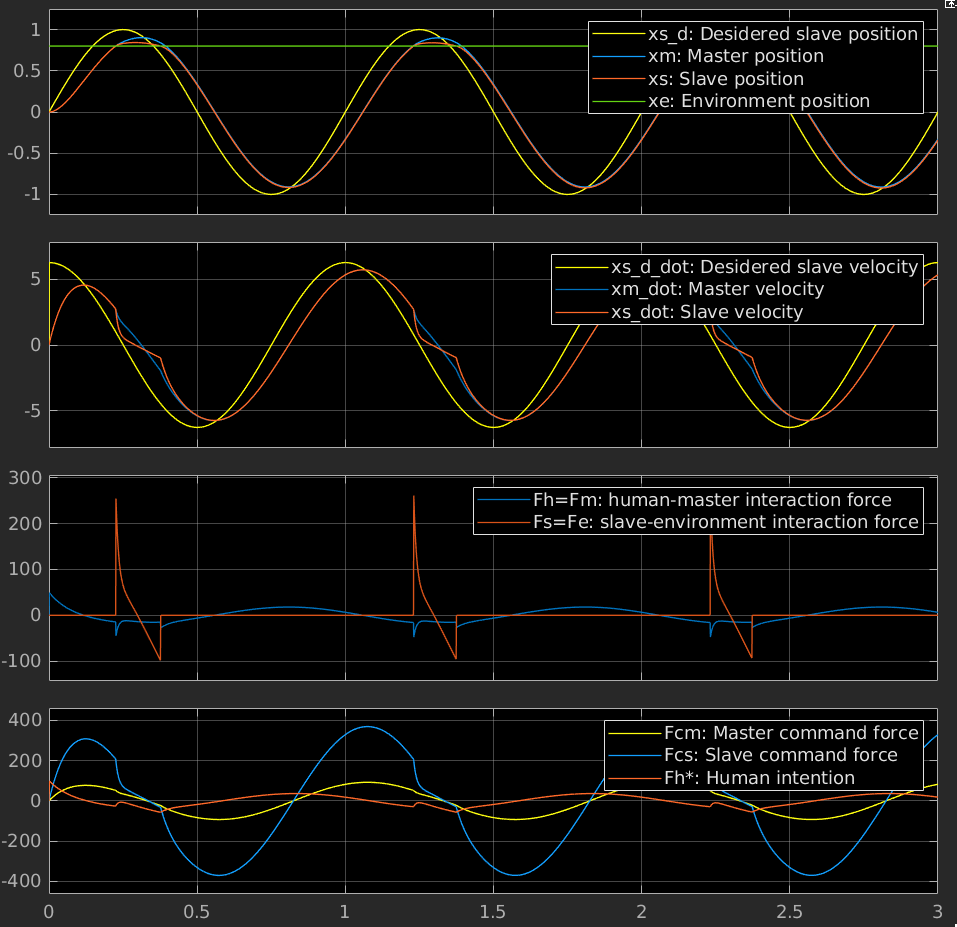
\includegraphics[keepaspectratio,width=\textwidth]{PFP_contact_nod}
\caption{3-channel P,F-P in contact.}
\label{fig:pfp_contact}
\end{figure}
\end{minipage}
\end{figure}

\newpage

\subsection{What happens if transportation delays are added in series to the coordinating controllers?}

\begin{figure}[H]
\begin{minipage}{0.5\textwidth}
\begin{figure}[H]
\centering
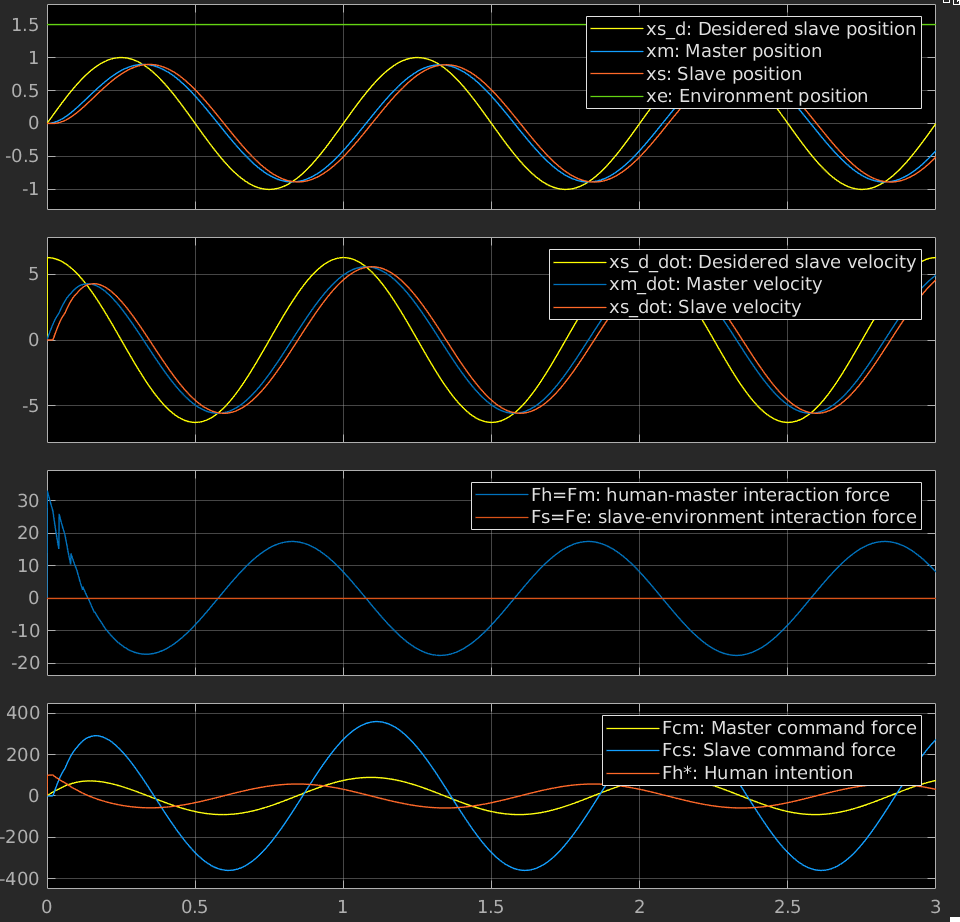
\includegraphics[keepaspectratio,width=\textwidth]{PP_d}
\caption{2-channel P-P in free motion with transportation delays.}
\label{fig:pp_d}
\end{figure}
\begin{figure}[H]
\centering
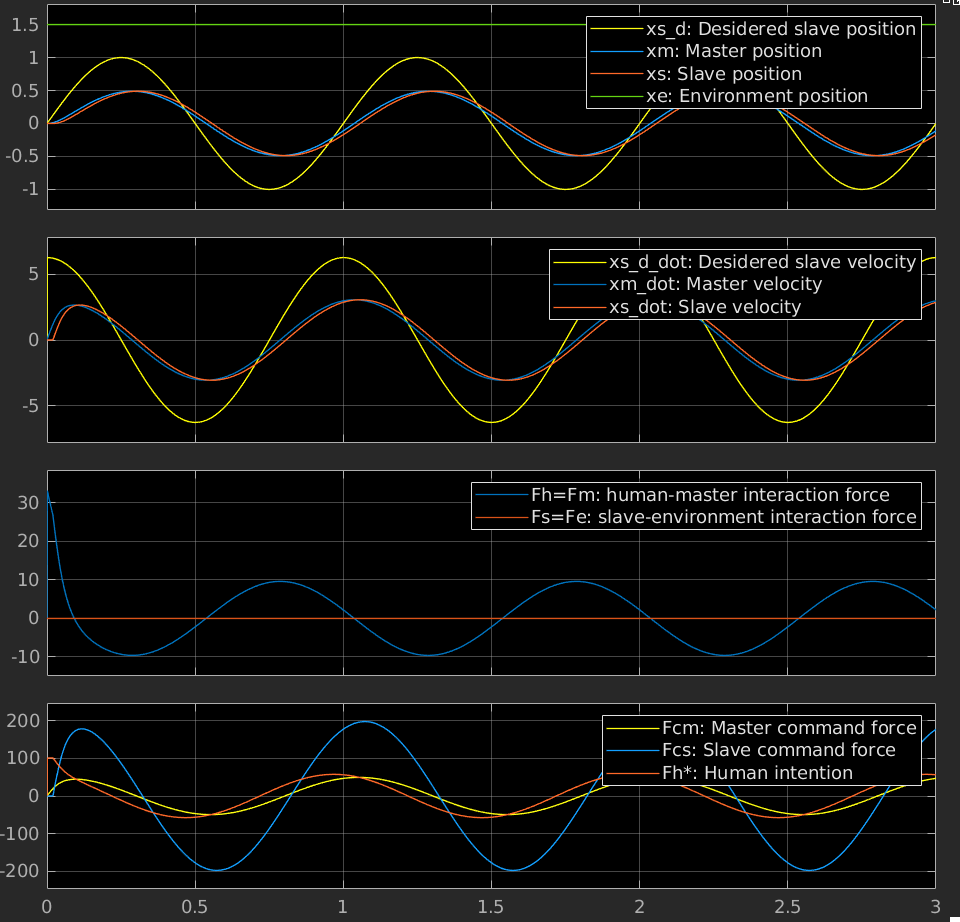
\includegraphics[keepaspectratio,width=\textwidth]{FP_d}
\caption{2-channel F-P in free motion with transportation delays.}
\label{fig:fp_d}
\end{figure}
\end{minipage}
\begin{minipage}{0.5\textwidth}
\begin{figure}[H]
\centering
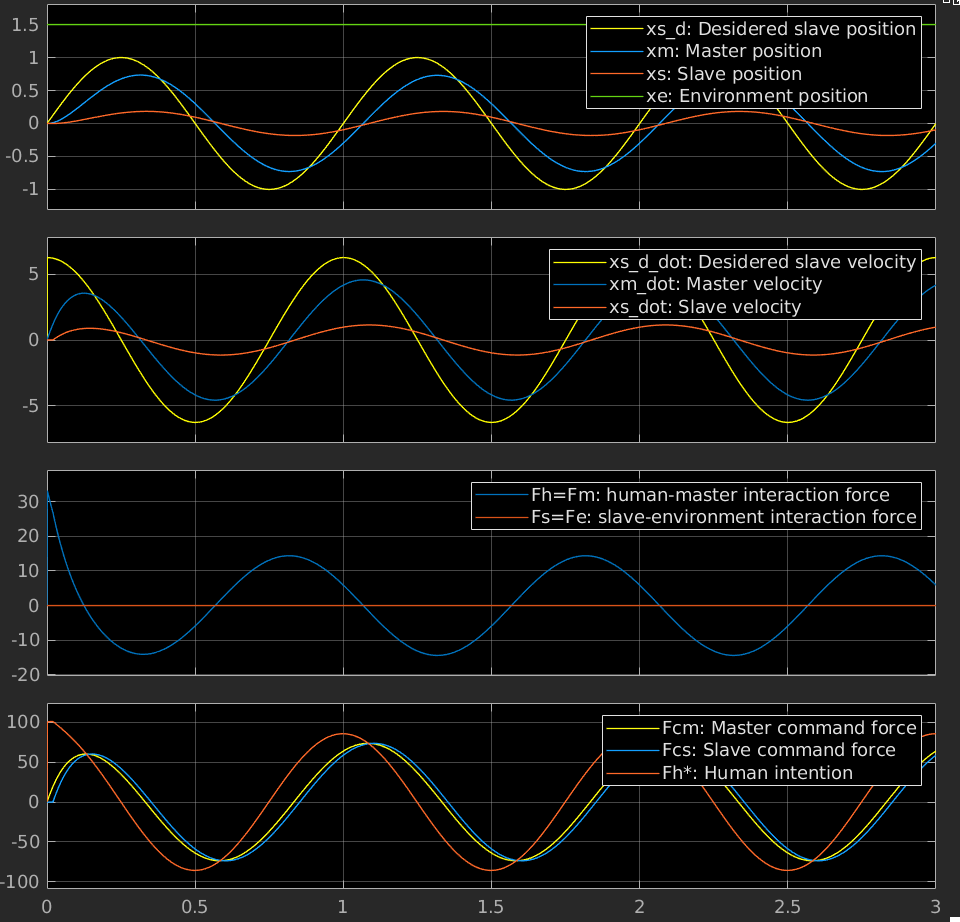
\includegraphics[keepaspectratio,width=\textwidth]{FF_d}
\caption{2-channel F-F in free motion with transportation delays.}
\label{fig:ff_d}
\end{figure}
\begin{figure}[H]
\centering
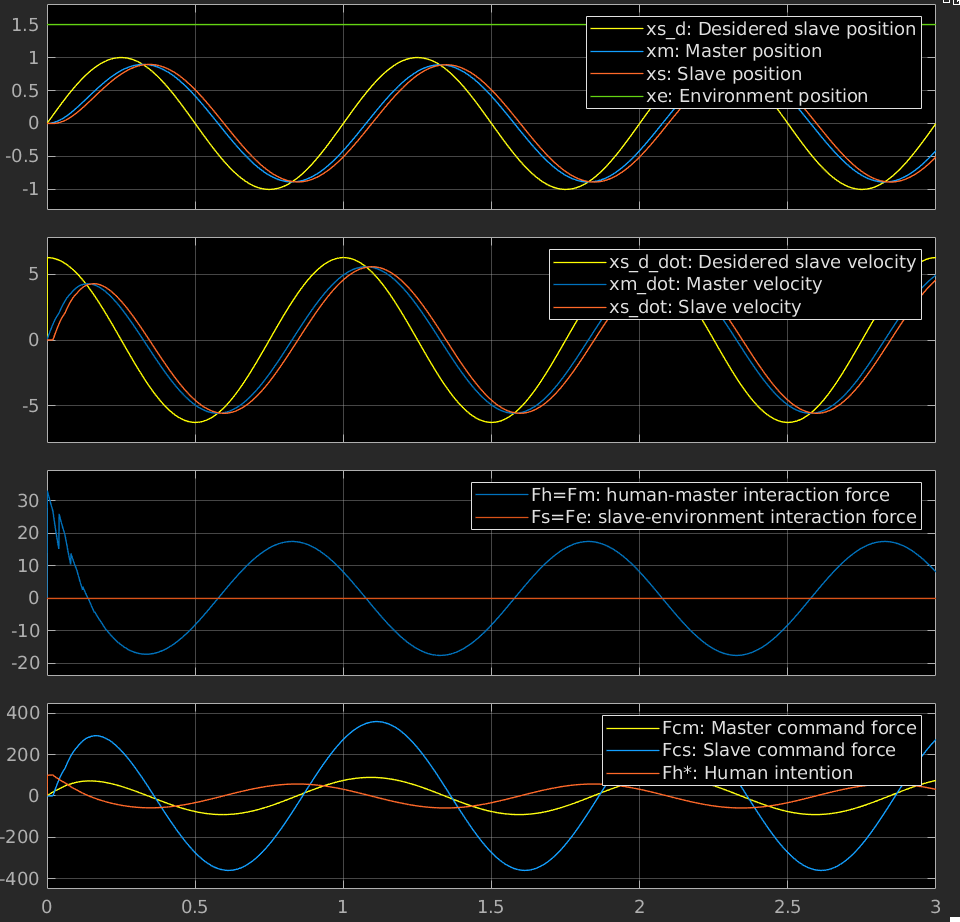
\includegraphics[keepaspectratio,width=\textwidth]{PFP_d}
\caption{3-channel P,F-P in free motion with transportation delays.}
\label{fig:pfp_d}
\end{figure}
\end{minipage}
\end{figure}

\newpage

\begin{figure}[H]
\begin{minipage}{0.5\textwidth}
\begin{figure}[H]
\centering
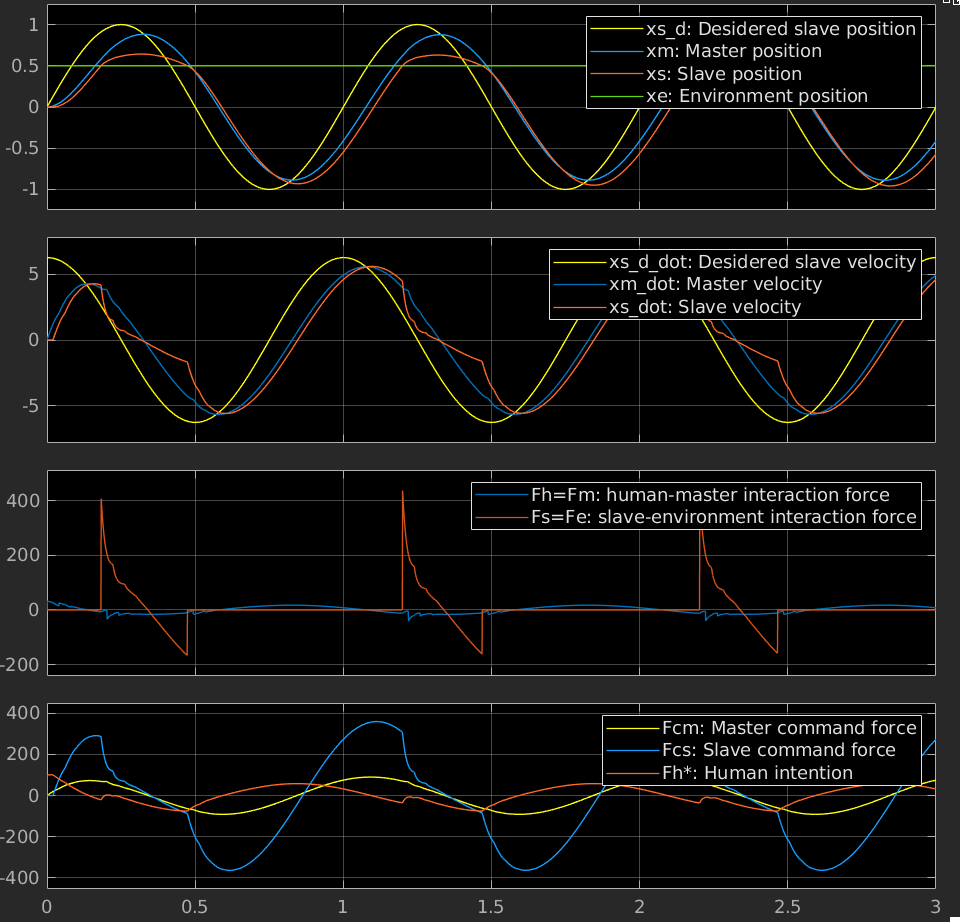
\includegraphics[keepaspectratio,width=\textwidth]{PP_contact_d}
\caption{2-channel P-P in contact with transportation delays.}
\label{fig:pp_contact_d}
\end{figure}
\begin{figure}[H]
\centering
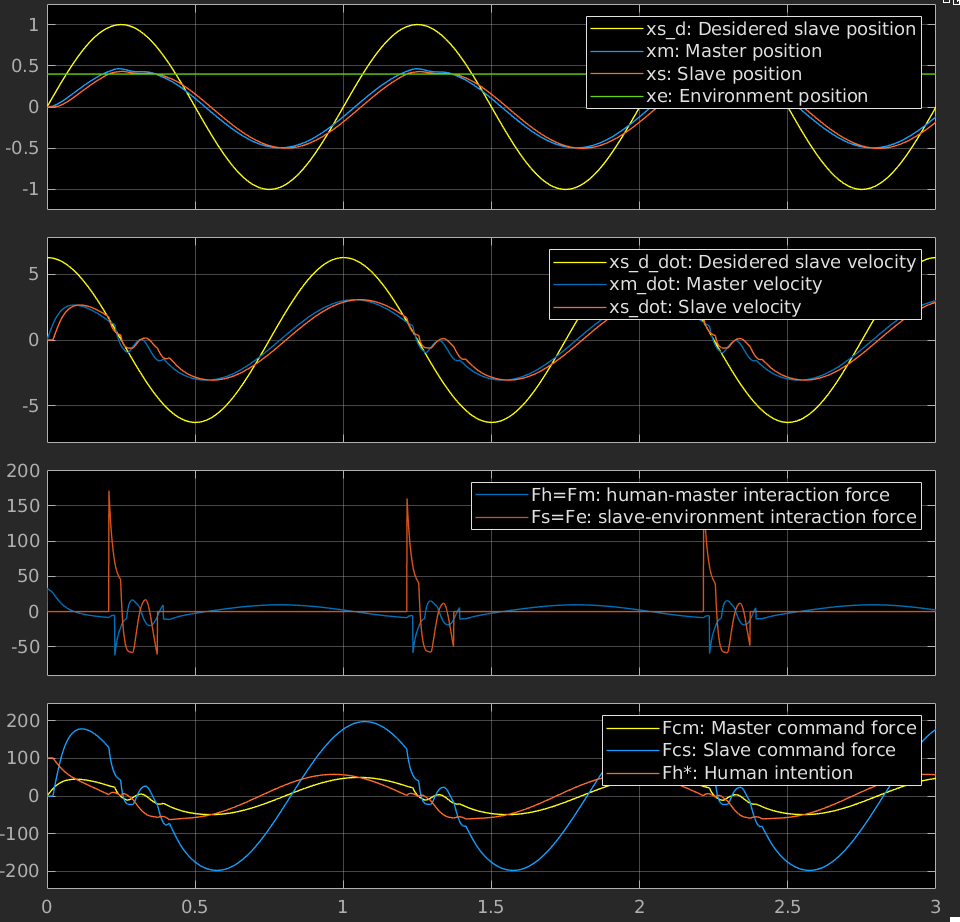
\includegraphics[keepaspectratio,width=\textwidth]{FP_contact_d}
\caption{2-channel F-P in contact with transportation delays.}
\label{fig:fp_contact_d}
\end{figure}
\end{minipage}
\begin{minipage}{0.5\textwidth}
\begin{figure}[H]
\centering
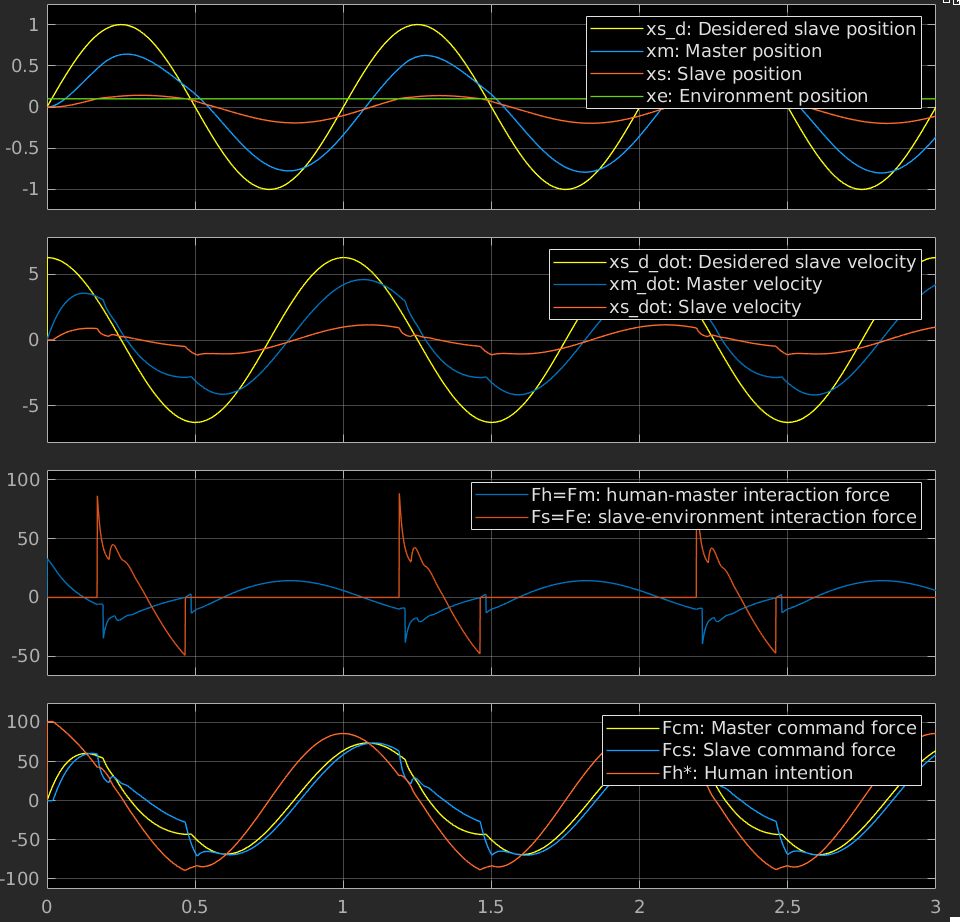
\includegraphics[keepaspectratio,width=\textwidth]{FF_contact_d}
\caption{2-channel F-F in contact with transportation delays.}
\label{fig:ff_contact_d}
\end{figure}
\begin{figure}[H]
\centering
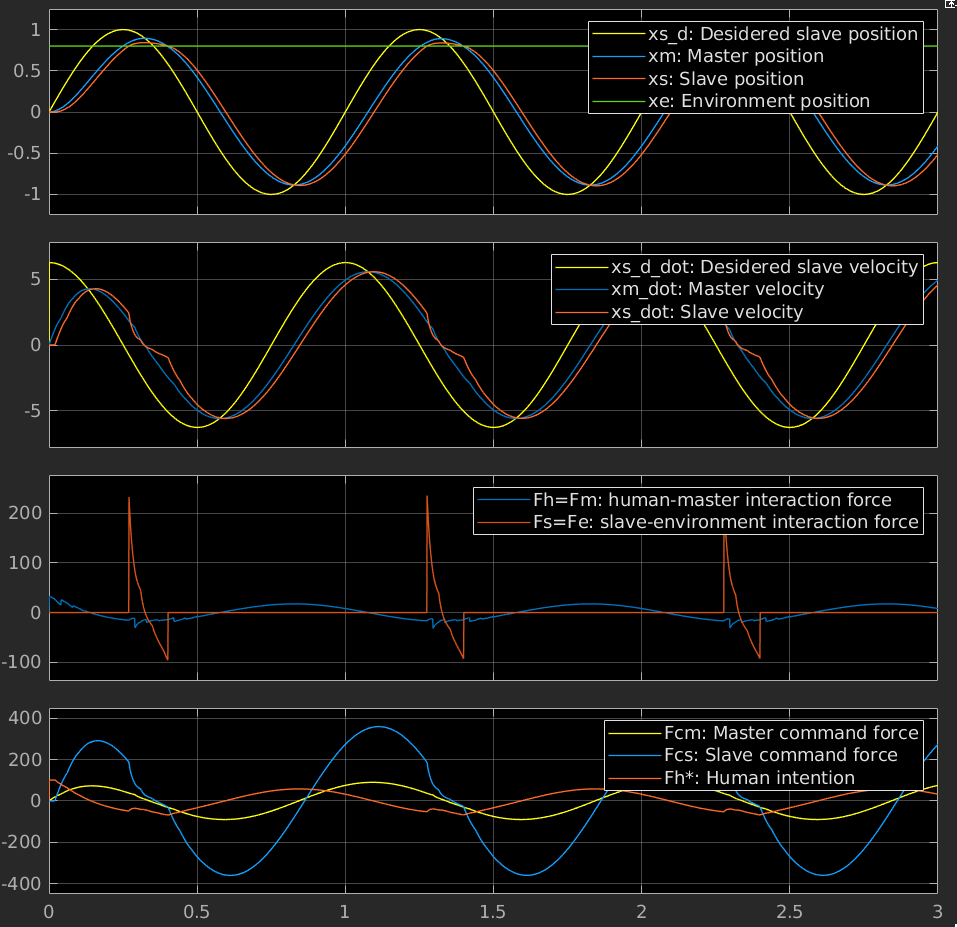
\includegraphics[keepaspectratio,width=\textwidth]{PFP_contact_d}
\caption{3-channel P,F-P in contact with transportation delays.}
\label{fig:pfp_contact_d}
\end{figure}
\end{minipage}
\end{figure}